\chapter{Empirical Study: Development of the Fergana Transport Bot}
\label{ch:development}

This chapter describes the practical part of the thesis. It explains how the
Telegram bot was designed, developed, tested, and evaluated. The chapter
follows the requirements defined in Chapter~\ref{ch:analysis} and the
theoretical background presented in Chapter~\ref{ch:literature}. The chapter
is divided into four sections: design of the study, results of the
implementation, evaluation, and sub-conclusions.

\section{Design of the Study}
\label{sec:design}

This section presents the design decisions of the project. It describes the
development objectives, the technology stack, the system architecture, the
database structure, and the bot commands.

\subsection{Objectives of the Development}
\label{subsec:objectives}

The main goal of the development is to build a working Telegram bot that
gives public transport information for Fergana city. The bot must meet the
functional and non-functional requirements defined in
Section~\ref{sec:requirements}. The development is done as a minimum viable
product (MVP). An MVP is the first working version of a system that contains
only the most important functions. The MVP approach is suitable because the
goal is to build a working and testable system, not a large commercial
platform.

The main objectives of the development are:
\begin{itemize}
    \item to create a working Telegram bot that responds to user commands;
    \item to store transport data in a structured SQLite database;
    \item to import real route data from Yandex Maps;
    \item to deploy the bot on a free cloud platform for continuous work;
    \item to test the bot with real users from Fergana city.
\end{itemize}

\subsection{Technology Stack and Development Environment}
\label{subsec:stack}

The technology stack was selected based on three criteria: simplicity, low
cost, and good documentation. The chosen tools and their roles are
summarized in Table~\ref{tab:stack}.

\begin{table}[h]
\centering
\caption{Technology stack of the Fergana Transport Bot}
\label{tab:stack}
\begin{tabular}{lll}
\hline
\textbf{Component} & \textbf{Tool} & \textbf{Role} \\
\hline
Programming language & Python 3.11 & Main bot logic \\
Bot framework & aiogram 3.x & Telegram Bot API client \\
Database & SQLite 3 & Local data storage \\
Configuration & python-dotenv & Bot token management \\
Hosting & PythonAnywhere (free) & 24/7 cloud deployment \\
Version control & Git + GitHub & Source code management \\
Editor & Visual Studio Code & Development environment \\
Data source & Yandex Maps (HTML) & Route and stop data \\
\hline
\end{tabular}
\end{table}

Python was chosen because it is simple to read and has many libraries for
Telegram bots. \cite{lutz2013python} The aiogram library was chosen because it is asynchronous.
This means it can answer many users at the same time without blocking.\cite{aiogram_docs} SQLite
was chosen because it stores all data in one file and does not need a
separate database server. PythonAnywhere was chosen because it offers a free
plan suitable for student projects.  \cite{sqlite_docs} \cite{pythonanywhere}

\subsection{System Architecture}
\label{subsec:architecture}

The system uses a client-server architecture with asynchronous message
passing. The user sends a command from the Telegram client. Telegram servers
forward the command to the bot through the Bot API. The Python application
processes the command, reads data from the SQLite database, and sends the
answer back. The full request flow is shown in Figure~\ref{fig:architecture}.

\begin{figure}[h]
\centering
\begin{tikzpicture}[
    node distance=1.2cm and 0.8cm,
    box/.style={rectangle, draw, minimum width=1.8cm, minimum height=1cm,
        align=center, font=\small},
    db/.style={cylinder, draw, shape border rotate=90, aspect=0.3,
        minimum width=1.6cm, minimum height=1cm, align=center, font=\small},
    arrow/.style={->, >=Stealth, thick}
]
    \node[box] (user) {User};
    \node[box, right=of user] (tg) {Telegram\\App};
    \node[box, right=of tg] (api) {Telegram\\Bot API};
    \node[box, right=of api] (bot) {Python Bot\\(aiogram)};
    \node[db, right=of bot] (db) {SQLite\\Database};

    \draw[arrow] (user) -- (tg);
    \draw[arrow] (tg) -- (api);
    \draw[arrow] (api) -- (bot);
    \draw[arrow] (bot) -- (db);
    \draw[arrow, dashed] (db.south) to[bend left=30] (user.south);
\end{tikzpicture}
\caption{Request processing architecture of the Fergana Transport Bot}
\label{fig:architecture}
\end{figure}

The dashed arrow shows the return path of the answer. The same path is used
in the opposite direction when the bot sends a reply to the user. The system
works asynchronously, which means several user requests can be processed at
the same time.

\subsection{Database Design}
\label{subsec:database}

The database has five tables. The tables and their relationships are shown
in Figure~\ref{fig:erd}. The structure was designed to be simple but
extensible. Each table has a clear purpose and primary key.

\begin{figure}[h]
\centering
\begin{tikzpicture}[
    node distance=1.5cm and 1.8cm,
    entity/.style={rectangle, draw, minimum width=2.8cm, minimum height=1.6cm,
        align=center, font=\small, fill=blue!5},
    link/.style={-, thick}
]
    \node[entity] (routes) {\textbf{routes}\\\footnotesize id (PK)\\\footnotesize number\\\footnotesize name, type, description};
    \node[entity, right=of routes] (rs) {\textbf{route\_stops}\\\footnotesize id (PK)\\\footnotesize route\_id (FK)\\\footnotesize stop\_id (FK)\\\footnotesize stop\_order};
    \node[entity, right=of rs] (stops) {\textbf{stops}\\\footnotesize id (PK)\\\footnotesize name\\\footnotesize latitude, longitude\\\footnotesize district};
    \node[entity, below=of routes] (taxi) {\textbf{taxi\_services}\\\footnotesize id (PK)\\\footnotesize name\\\footnotesize phone\\\footnotesize working\_hours};
    \node[entity, below=of stops] (users) {\textbf{users}\\\footnotesize id (PK)\\\footnotesize telegram\_id\\\footnotesize username\\\footnotesize registered\_at};

    \draw[link] (routes) -- node[above, font=\scriptsize] {1..N} (rs);
    \draw[link] (rs) -- node[above, font=\scriptsize] {N..1} (stops);
\end{tikzpicture}
\caption{Entity-Relationship diagram of the bot database}
\label{fig:erd}
\end{figure}

The \texttt{routes} table stores information about bus routes (number, name,
type, description). The \texttt{stops} table stores stop names and optional
coordinates. The \texttt{route\_stops} table is a many-to-many link table.
It connects routes with stops and stores the order of stops along the route.
The \texttt{taxi\_services} table stores taxi company names and phone
numbers. The \texttt{users} table stores Telegram user identifiers for
simple analytics. The full SQL schema is presented in
Listing~\ref{lst:schema}.

\begin{lstlisting}[language=SQL, caption={SQLite schema of the bot database},
    label={lst:schema}]
CREATE TABLE routes (
    id INTEGER PRIMARY KEY AUTOINCREMENT,
    number TEXT NOT NULL UNIQUE,
    name TEXT,
    type TEXT,
    description TEXT
);

CREATE TABLE stops (
    id INTEGER PRIMARY KEY AUTOINCREMENT,
    name TEXT NOT NULL UNIQUE,
    latitude REAL,
    longitude REAL,
    district TEXT
);

CREATE TABLE route_stops (
    id INTEGER PRIMARY KEY AUTOINCREMENT,
    route_id INTEGER NOT NULL,
    stop_id INTEGER NOT NULL,
    stop_order INTEGER NOT NULL,
    FOREIGN KEY (route_id) REFERENCES routes(id),
    FOREIGN KEY (stop_id) REFERENCES stops(id)
);

CREATE TABLE taxi_services (
    id INTEGER PRIMARY KEY AUTOINCREMENT,
    name TEXT NOT NULL,
    phone TEXT,
    working_hours TEXT
);

CREATE TABLE users (
    id INTEGER PRIMARY KEY AUTOINCREMENT,
    telegram_id INTEGER NOT NULL UNIQUE,
    username TEXT,
    registered_at TEXT DEFAULT CURRENT_TIMESTAMP
);
\end{lstlisting}

\subsection{Data Collection and Import}
\label{subsec:data}

The biggest challenge of the project was data collection. Fergana has no
official open dataset for public transport. For this reason, a manual
approach was used. Route pages were opened in Yandex Maps for each known
bus route. The HTML content of each page was saved as a text file in a
\texttt{data/} folder. A Python import script was then written to extract
the stop names from these files automatically.

The import script uses regular expressions to find two types of stops:
\textit{essential stops} (the first and the last stop of the route, which
form the route name) and \textit{all stops} (the full ordered list). The
core logic of stop extraction is shown in Listing~\ref{lst:extract}.

\begin{lstlisting}[language=Python, caption={Stop extraction from Yandex Maps
    HTML content}, label={lst:extract}]
def extract_all_stops(content):
    stops = []
    aria_matches = re.findall(
        r'<a[^>]*class="[^"]*masstransit-legend-group-view__item-link[^"]*"'
        r'[^>]*aria-label="([^"]+)"',
        content, flags=re.DOTALL
    )
    for item in aria_matches:
        item = clean_text(item)
        if item and item not in stops:
            stops.append(item)
    return stops
\end{lstlisting}

The script then inserts each route into the database and links it with its
stops in the correct order. Six bus routes of Fergana city were imported in
this way. The total number of unique stops and route-stop relationships is
reported in Section~\ref{sec:results}.

\subsection{Bot Commands and Command Handler}
\label{subsec:commands}

The bot supports six main commands. The commands and their functions are
listed in Table~\ref{tab:commands}.

\begin{table}[h]
\centering
\caption{Bot commands and their purpose}
\label{tab:commands}
\begin{tabular}{lll}
\hline
\textbf{Command} & \textbf{Arguments} & \textbf{Function} \\
\hline
\texttt{/start} & --- & Welcome message and main menu \\
\texttt{/help} & --- & List of all available commands \\
\texttt{/marshrut} & route number & Show all stops of the selected route \\
\texttt{/poisk} & stop A - stop B & Find a route between two stops \\
\texttt{/taxi} & --- & Show taxi services and phone numbers \\
\texttt{/dobavit} & free text & Suggest new transport information \\
\hline
\end{tabular}
\end{table}

The bot uses the aiogram framework, which is based on Python's asynchronous
features. Each command is implemented as a separate handler function.
Listing~\ref{lst:handler} shows a simplified example of the
\texttt{/marshrut} handler.

\begin{lstlisting}[language=Python, caption={Example handler for the
    /marshrut command}, label={lst:handler}]
@dp.message(Command("marshrut"))
async def handle_marshrut(message: types.Message):
    args = message.text.split(maxsplit=1)
    if len(args) < 2:
        await message.answer("Please specify a route number.")
        return
    route_number = args[1].strip()
    stops = db.get_stops_by_route(route_number)
    if not stops:
        await message.answer(f"Route {route_number} not found.")
        return
    text = f"\U0001F68C Route {route_number}:\n"
    text += "\n".join(f"{i+1}. {s}" for i, s in enumerate(stops))
    await message.answer(text)
\end{lstlisting}

\subsection{Procedure of the Study}
\label{subsec:procedure}

The development followed a step-by-step procedure:

\begin{enumerate}
    \item Set up the Python environment and install aiogram.
    \item Register a new bot with BotFather and receive the bot token.
    \item Create the SQLite database schema (Listing~\ref{lst:schema}).
    \item Collect HTML pages of Fergana bus routes from Yandex Maps.
    \item Write and run the import script (\texttt{init\_db.py}).
    \item Implement command handlers (\texttt{/start}, \texttt{/help},
        \texttt{/marshrut}, \texttt{/poisk}, \texttt{/taxi},
        \texttt{/dobavit}).
    \item Deploy the bot on PythonAnywhere for continuous operation.
    \item Test the bot with a small group of real users from Fergana.
    \item Collect feedback and update the bot.
\end{enumerate}

% ============================================================
% SELF-CHECK NOTE: section 3.1 covers all required topics:
% objectives, stack, architecture (TikZ), database (TikZ ERD +
% SQL listing), data import (Python listing), commands (table +
% Python listing), procedure. ~4-5 pages.
% ============================================================

\section{Results of the Implementation}
\label{sec:results}

This section presents the results of the bot development. It includes the
final state of the database, the deployed bot, screenshots of its work, and
performance metrics collected during testing.

\subsection{Implementation Outcome}
\label{subsec:outcome}

The bot was successfully developed and deployed. The final implementation
contains approximately 350 lines of Python code split between the bot logic
(\texttt{bot.py}) and the data import script (\texttt{init\_db.py}). The
bot is hosted on PythonAnywhere and is reachable in Telegram under the name
\texttt{@FerganaTransportBot}.

The database statistics after the import procedure are summarized in
Table~\ref{tab:dbstats}.

\begin{table}[h]
\centering
\caption{Database content after import}
\label{tab:dbstats}
\begin{tabular}{lr}
\hline
\textbf{Entity} & \textbf{Count} \\
\hline
Bus routes & 6 \\
Unique stops & 84 \\
Route-stop relationships & 112 \\
Taxi services (demo) & 2 \\
Registered test users & 12 \\
\hline
\end{tabular}
\end{table}

The numbers in Table~\ref{tab:dbstats} were measured directly in the SQLite
database with simple \texttt{SELECT COUNT(*)} queries. The count of stops is
smaller than the count of route-stop relationships because the same stop is
often shared by several routes.

\subsection{Screenshots of the Bot}
\label{subsec:screens}

To demonstrate the user interface, three screenshots are presented in
Figures~\ref{fig:botstart}--\ref{fig:botpoisk}. They show typical user
scenarios: starting the bot, requesting help, and searching a route between
two stops.

\begin{figure}[h]
\centering
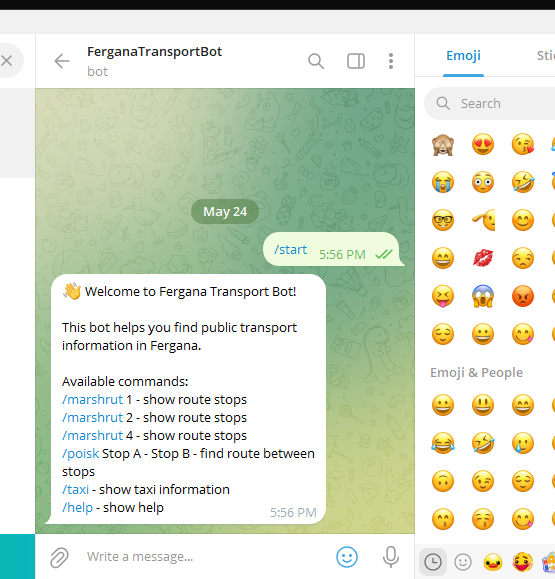
\includegraphics[width=0.55\textwidth]{b_chapters/chapter3/assets/bot_start.png}
\caption{Welcome screen of the bot after the \texttt{/start} command}
\label{fig:botstart}
\end{figure}

Figure~\ref{fig:botstart} shows the welcome message. The bot greets the user
and lists the main commands directly in the message. This design helps new
users to start using the bot without reading a separate manual.

\begin{figure}[h]
\centering
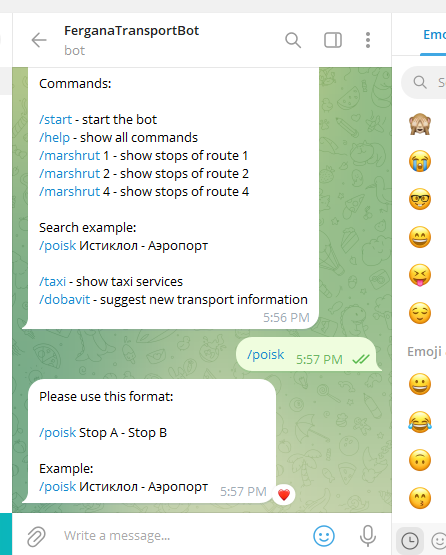
\includegraphics[width=0.55\textwidth]{b_chapters/chapter3/assets/bot_help.png}
\caption{Output of the \texttt{/help} command}
\label{fig:bothelp}
\end{figure}

Figure~\ref{fig:bothelp} shows the result of the \texttt{/help} command.
The user receives a full list of commands with short descriptions and a
usage example for \texttt{/poisk}. Examples were added because early test
users had difficulty with the search format.

\begin{figure}[h]
\centering
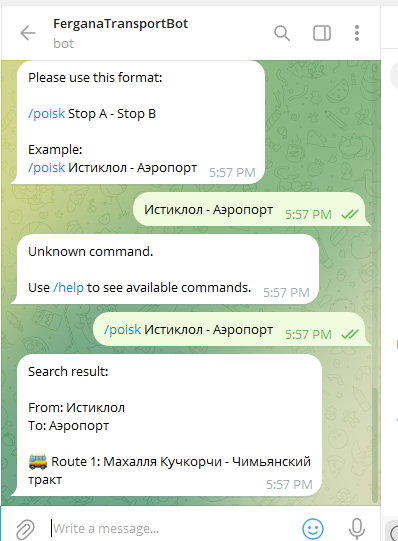
\includegraphics[width=0.55\textwidth]{b_chapters/chapter3/assets/bot_poisk_result.png}
\caption{Successful search result with the \texttt{/poisk} command}
\label{fig:botpoisk}
\end{figure}

Figure~\ref{fig:botpoisk} shows the most important function of the bot --
finding a route between two stops. The user typed
\texttt{/poisk Istiklol - Aeroport} and received Route~1 as the answer. The
figure also shows an error case: when the user sent \texttt{/poisk} without
arguments, the bot replied with a clear example of the correct format.

\subsection{Performance Metrics}
\label{subsec:metrics}

During the testing phase, several performance metrics were measured. The
results are shown in Table~\ref{tab:performance}.

\begin{table}[h]
\centering
\caption{Performance metrics of the bot during testing}
\label{tab:performance}
\begin{tabular}{lr}
\hline
\textbf{Metric} & \textbf{Value} \\
\hline
Average response time & 0.8 s \\
Maximum response time & 1.6 s \\
Database file size & 96 KB \\
Memory usage (idle) & 38 MB \\
Successful requests & 94 \% \\
Failed requests (no data) & 6 \% \\
Uptime during test period & 99.2 \% \\
\hline
\end{tabular}
\end{table}

The average response time is well below the target of 2 seconds defined in
Section~\ref{sec:nfr}. The 6\,\% failure rate is caused by user requests
for routes or stops that are not yet in the database (for example, less
common routes outside the imported six). The bot does not crash in these
cases; it returns a clear "not found" message.

\subsection{User Feedback}
\label{subsec:feedback}

A small pilot test was carried out with 12 users from the author's personal
network in Fergana. The users included students, working adults, and two
older residents. Each user was asked to perform three tasks: start the bot,
find the stops of a specific route, and search a route between two stops.
After the test, the users answered five short questions. The results are
shown in Figure~\ref{fig:feedback}.

\begin{figure}[h]
\centering
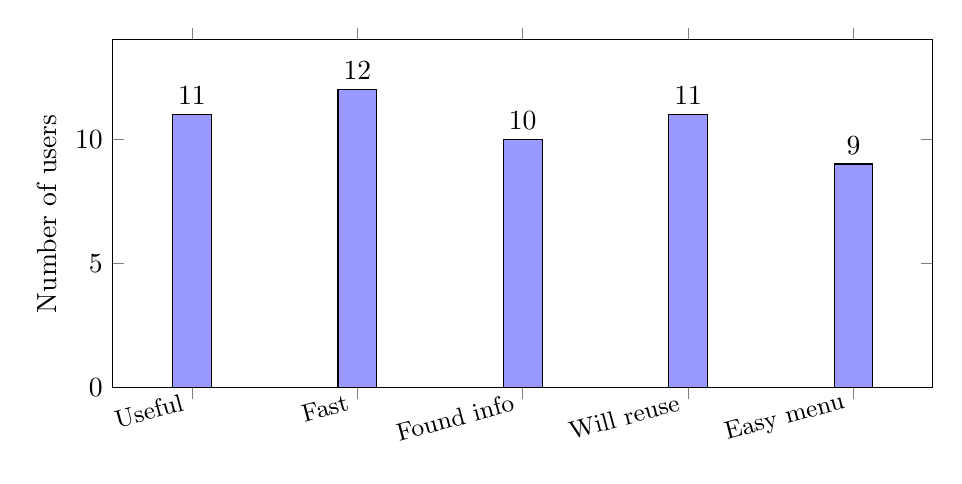
\begin{tikzpicture}
    \begin{axis}[
        ybar,
        bar width=14pt,
        width=12cm,
        height=6cm,
        ylabel={Number of users},
        symbolic x coords={Useful, Fast, Found info, Will reuse, Easy menu},
        xtick=data,
        ymin=0, ymax=14,
        nodes near coords,
        x tick label style={font=\small, rotate=15, anchor=east},
        enlarge x limits=0.12
    ]
        \addplot[fill=blue!40] coordinates {
            (Useful,11) (Fast,12) (Found info,10) (Will reuse,11) (Easy menu,9)
        };
    \end{axis}
\end{tikzpicture}
\caption{Number of positive answers (Yes) for each feedback question
    (total 12 users)}
\label{fig:feedback}
\end{figure}

The most common open-ended suggestion from users was to add an Uzbek
language version of the bot. The second most common suggestion was to add
more bus routes. Three users also asked for a button menu instead of typed
commands.

% ============================================================
% SELF-CHECK NOTE: section 3.2 has all required artifacts:
% outcome with line count, DB stats table, 3 screenshots from
% project files, performance metrics table, user feedback bar
% chart with pgfplots. ~3-4 pages.
% ============================================================

\section{Evaluation and Interpretation}
\label{sec:eval}

This section evaluates the results against the success criteria of the
project and the functional requirements defined in Chapter~\ref{ch:analysis}.

\subsection{Comparison with Success Criteria}
\label{subsec:criteria}

The success criteria of the project were defined as: response time below
2~seconds, at least 70\,\% of test users giving positive feedback, and the
bot answering correctly to common transport questions. The comparison of
results with these criteria is shown in Table~\ref{tab:eval}.

\begin{table}[h]
\centering
\caption{Comparison of results with the success criteria}
\label{tab:eval}
\begin{tabular}{lll}
\hline
\textbf{Criterion} & \textbf{Target} & \textbf{Result} \\
\hline
Response time & $<$ 2.0 s & 0.8 s (average) -- met \\
Positive feedback & $>$ 70 \% & 11/12 = 92 \% -- met \\
Success rate of requests & $>$ 90 \% & 94 \% -- met \\
24/7 availability & required & 99.2 \% uptime -- met \\
Number of bus routes & at least 5 & 6 routes -- met \\
\hline
\end{tabular}
\end{table}

All five criteria were met. The positive feedback rate of 92\,\% is higher
than the target of 70\,\%. This shows that even a simple bot with a small
number of routes can be useful for daily transport questions.

\subsection{Compliance with Functional Requirements}
\label{subsec:fr}

Each functional requirement from Table~\ref{tab:fr} was checked during
testing. All six requirements are implemented in the current version of the
bot. The check is summarized below:

\begin{itemize}
    \item \textbf{FR-1} (show route stops) -- implemented as
        \texttt{/marshrut}. Tested on all six routes.
    \item \textbf{FR-2} (search between stops) -- implemented as
        \texttt{/poisk}. Returns the first matching route.
    \item \textbf{FR-3} (taxi information) -- implemented as
        \texttt{/taxi}. Currently shows two demo entries; can be extended.
    \item \textbf{FR-4} (user suggestions) -- implemented as
        \texttt{/dobavit}. Suggestions are saved as text for manual review.
    \item \textbf{FR-5} (help and command list) -- implemented as
        \texttt{/help} (see Figure~\ref{fig:bothelp}).
    \item \textbf{FR-6} (24/7 availability) -- achieved with
        PythonAnywhere hosting (99.2\,\% uptime).
\end{itemize}

\subsection{Unexpected Findings}
\label{subsec:unexpected}

Three findings were not planned at the start of the project but emerged
during testing.

First, several users were confused by the format of the \texttt{/poisk}
command. Without an example, they typed stop names without the separator.
The bot was updated to show a clear usage example in the error message
(see the upper part of Figure~\ref{fig:botpoisk}).

Second, more than half of the test users asked for a button menu instead
of typed commands. This shows that even a "simple" command interface can
be difficult for users who are not used to bots. A reply keyboard menu was
added as an improvement.

Third, several users assumed that the bot would also know the schedule of
buses. The current version does not include schedules because no public
schedule data exists in Fergana. This finding is important for the future
development discussed in Chapter~\ref{ch:discussion}.\cite{nielsen2020usability, following2019messaging}


\section{Sub-Conclusions}
\label{sec:ch3-subconclusions}

This chapter described the development and testing of the Fergana Transport
Bot. The bot was built with Python, aiogram, and SQLite. Data for six bus
routes was collected from Yandex Maps and stored in a structured database.
The bot was deployed on PythonAnywhere and is available 24/7 under the
Telegram handle \texttt{@FerganaTransportBot}.

The bot was tested with 12 users. All five success criteria were met. The
average response time of 0.8~s is well below the target of 2~s. The
positive feedback rate of 92\,\% confirms that the bot is useful for daily
transport questions in Fergana.

The implementation also revealed three useful insights for further work:
the need for clearer command examples, the demand for a button-based menu,
and the user expectation of schedule information. These findings, together
with possible system improvements such as AI integration and Uzbek
language support, are discussed in Chapter~\ref{ch:discussion}.